\mode*

\begin{frame}{Limites de la parallélisation}
  \vFill
  \begin{center}
      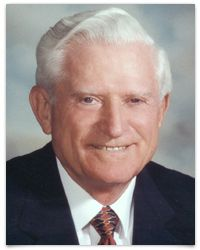
\includegraphics[height=4cm]{gene_amdahl}\\
      Gene M. Amdahl
    \end{center}
  \vFill
  \begin{citing}
  \item[A67] Gene M. Amdahl. \textit{Validity of the Single Processor Approach to Achieving Large-Scale Computing Capabilities.} AFIPS (1967)
  \end{citing}
\end{frame}
 
\begin{frame}{Limites de la parallélisation}
  \begin{alertblock}{Question}
    \begin{itemize}
    \item Un sondeur a besoin de 22 jours pour interroger 1000 sondés.
    \item Combien de temps faut-il à 22 sondeurs pour faire le même sondage ?
    \end{itemize}
  \end{alertblock}
  \pause
  \begin{alertblock}{Question}
    \begin{itemize}
    \item Une éléphante a besoin de 22 mois pour donner la vie.
    \item Combien de temps faut-il à 22 éléphantes pour faire le même éléphanteau ?
    \end{itemize}
  \end{alertblock}
  \pause
  \begin{block}{Cas géneral}
    \begin{itemize}
    \item Une proportion $p$ du programme peut être parallélisée.
    \item Une proportion $1-p$ ne le peut pas.
    \end{itemize}
  \end{block}
\end{frame}
 
\begin{frame}{La loi d'Amdahl}
    \begin{description}
    \item[$p$: ] Proportion du programme parallélisable 
    \item[$T(n)$: ] Temps nécessaire à $n$ threads
    \item[$S(n)$: ] Accélération (Speedup) $S(n) = \frac{T(1)}{T(n)}$ 
    \end{description}
    \pause
    \hspace{\fill}
    \begin{minipage}{.6\textwidth}
    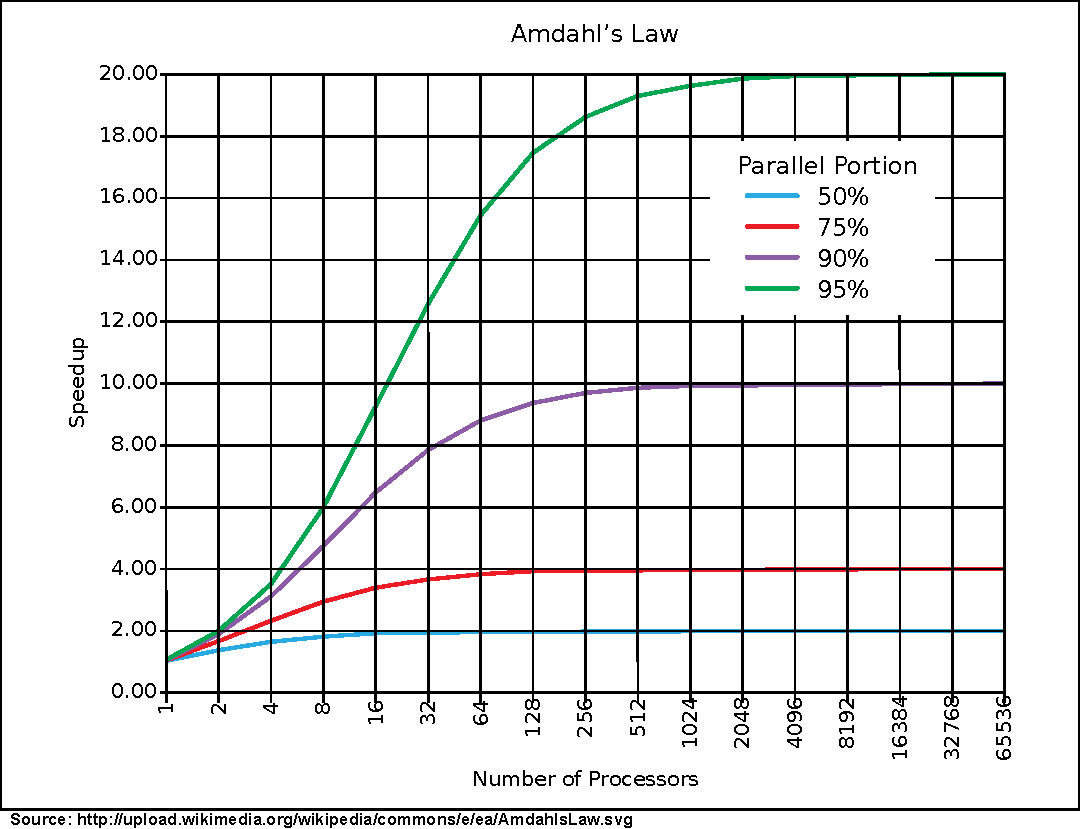
\includegraphics[width=\textwidth]{amdahl-law}
    \end{minipage}
    \hspace{\fill}
    \begin{minipage}{.35\textwidth}
      \vspace{-1cm}
      $$
      \begin{array}{rcl}
        \displaystyle S(n) &\displaystyle =& \displaystyle \frac{1}{1-p + \frac{p}{n}}\\
        \\
        \displaystyle S(n) &\displaystyle <& \displaystyle\frac{1}{1-p}\\
        \\
        \displaystyle \lim_{n\rightarrow \infty} S(n) &\displaystyle =& \displaystyle \frac{1}{1-p}
      \end{array}
      $$
    \end{minipage}
    \hspace{\fill}
\end{frame}
 
\begin{frame}{Limites de la loi d'Amdahl}
  \begin{block}{Hypothèses cachées :}
    \begin{itemize}
    \item Parallélisation imparfaite
    \begin{itemize}
    \item $p$ dépend des données (loi de Gustafson)
    \item $p$ dépend de l'algorithme
    \end{itemize}
    $$S_p(n) \le n$$
  \item Synchronisation non-parallélisable
    \begin{itemize}
    \item Gestion de la concurrence
    \end{itemize}
    $$S_c(n) \le 1$$
    \end{itemize}
  \end{block}
  \begin{block}{Formule plus réaliste}
    $$
    S(n) = \frac{1}{\frac{1-p}{S_c(n)} + \frac{p}{S_p(n)}} \le \frac{1}{1-p + \frac{p}{n}}
    $$
    \begin{center}
      \alert{Mesurez vos performances !}
    \end{center}
  \end{block}
\end{frame}



\mode<all>


